\documentclass[annotation,times,page4]{itmo-student-thesis}

%% Опции пакета:
%% - annotation - если есть, генерируется аннотация, иначе не генерируется
%% - times - делает все шрифтом Times New Roman, требует пакета pscyr.
%% - page4 - начинает нумерацию оглавления с четвертой, а не с третьей страницы

%% Данные пакеты необязательны к использованию в бакалаврских/магистерских
%% Они нужны для иллюстративных целей
%% Начало
\usepackage{tikz}
\usetikzlibrary{arrows}
\usepackage{filecontents}
%% Указываем файл с библиографией.
\addbibresource{master-thesis.bib}

\begin{document}

\studygroup{М4238}
\title{Выделение групп пользователей в социaльных медиа по их интересам и поведению на основе множества источников данных}
\author{Дмитриев С.С.}
\supervisor{Фильченков А.А.}
\supervisordegree{кандидат технических наук, доцент}
\publishyear{2016}

%% Транслируется в "Направление и задача исследований"
\researchdirections{Целью данного исследования является создание алгоритма выделения групп пользователей социальных сетей на основе их социальных связей и поведения в социальных сетях}

%% Транслируется в "Проектная и исследовательская часть"
\researchpart{В рамках данной работы предложен подход, позволяющий выделять подгруппы у выбранной группы пользователей в социальных сетях, основывающийся на социальных связях и видимом поведении на публичных страницах. В основе предложенного подхода лежат несколько методов и концепций: представление социальных связей в виде графа, случайные марковские поля, а так же семантический анализ. В качестве примера использования подхода взята группа футбольных болельщиков, и подгруппа радикальных футбольных болельщиков. Были использованы данные пользователей из социальной сети Vk.com. Достигнуты следующие показатели для группы футбольных болельщиков: точность 84\%, $f$-мера 0.46. Данный подход нов и так же может применятся для других групп и подгрупп пользователей.}

%% Транслируется в "Экономическая часть"
\economicpart{Данная работа не прополагает извлечения экономической выгоды из полученных результатов}

%% Транслируется в "Характеристика вопросов экологии, техники безопасности"
\ecologypart{Результатом работы является программный продукт, не нарушающий 
требования экологической безопасности.

}

%% Транслируется в "Новизна полученных результатов"
\novelty{В рамках описываемого исследования представлен подход, позволяющий определять принадлежность пользователя к определенной группе на основе его социальных связей и публичного поведения в социальной сети. Полученный подход является способом построения модели, не применявшимся для решения подобной задачи ранее. }

%% Транслируется в "Является ли работа продолжением курсовых проектов, есть ли публикации"
\cwpublications{Работа не является продолжением курсовых проектов. На тему диссертации имеются публикации. Дмитриев С. С. Выделение группы радикальных футбольных болельщиков в социальных медиа по их интересам и поведению на примере сети Vk.com //Материалы всероссийской научной конференции по проблемам информатики СПИСОК-2016 - 2016. - принято в печать.}

%% Транслируется в "Практическая ценность работы. Рекомендации по внедрению"
\practicalimplications{Полученный алгоритм дает возможность определить является ли член выбранной группы так же членом ее подможества. Это может быть использовано правоохранительными органами, т.к. алгоритм позволяет выделить, например подгруппы, склонные к бандитизму, пользователей потенциально более способных на совершение незаконных действий, нежели среднестатистический пользователь. Так же алгоритм может быть использован для усовершенствования таргетированной рекламы, например для выделения подгруппы фанатов определенного брэнда из группы его покупателей.}

%% Эта команда генерирует титульный лист и аннотацию.
\makemastertitle

%% Оглавление
\tableofcontents

%% Макрос для введения. Совместим со старым стилевиком.
\startprefacepage

Последнее время социальные медиа набрали огромную популярность. Такие сайты как Facebook.com\footnote{https://facebook.com}, Vk.com\footnote{https://vk.com}, Twitter.com,\footnote{https://twitter.com} обладают огромной аудиторией. Совокупный размер аудитории существующих социальных сетей составляет более двух миллиардов пользователей, и их число постоянно растет. Они создают огромные массы контента, состоящего из их мнений и точек зрения. Так в течении суток на Facebook.com более 4.5 миллиардов раз пользователи ставят лайки, оставляют более 700 тысяч публичных комментариев, публикуют более 100 миллионов фотографий\footnote{https://zephoria.com/top-15-valuable-facebook-statistics/}. Однако содержание этой информации в основном остается не использованным. Тогда как оно может быть крайне важным.

Такие данные могут быть использованы для определения интересов, предпочтений и иных личных свойств пользователя. Часть подобной информации, пол, возраст,  местоположение, увлечения, может быть указана в профиле пользователя. Однако, зачастую, такиe данные могут быть неполными, а иногда и неверными. А некоторые признаки, например, вероисповедание, политические взгляды или же принадлежность к неким общественным движениям обычно опускаются. Из-за этой неполноты возникает задача восстановления информации о пользователе.

Получение таких данных может быть полезно как бизнесу, так и государству~\cite{ramakrishnan2014beating}. Используя восстановленные характеристики, можно уточнять таргетированную рекламу~\cite{swearingen2001beyond}. Имея дополнительные данные об увлечениях людей, можно определять возможных преступников, что позволит предотвращать возможные нарушения или же прогнозировать конфликты~\cite{grothoff2016nsa}.

Существует множество исследований о восстановлении данных, явно неуказанных в профилях пользователей~\cite{blachnio2015facebook, schwartz2013personality, turdakov2013opredelenie, peersman2011predicting}. В них показано, что на основе информации о пользователе, его поведении в социальном медиа, можно с высокой точностью восстановить некоторые характеристики. 
Отдельной задачей стоит определения принадлежности пользователя к определенной группе, такой как, например, группа консерваторов или же группа любителей продукции Apple. Для решения  этой задачи часто используют данные о социальных связях пользователей. Показано, что они влияют на поведение человека, на его взгляды~\cite{trusov2010determining, bond201261}. 

В описываемом исследовании представлен подход для выделения подгруппы пользователей из определенной группы пользователей. Работа предложенного алгоритма продемонстрирована на примерe выделения подгруппы радикальных футбольных фанатов из группы футбольных болельщиков. Предполагается, что описываемый подход может быть использован на других группах и подгруппах пользователей различных социальных медиа.

%% Начало содержательной части.
\chapter{Обзор предметной области}
В данной главе описаны основные понятия, использующиеся в предметной области.

В разделе 1.1 описана задача о восстановлении характеристик пользователя, основные трудности, возникающие при решении этой задачи. 

В разделе 1.2 рассмотрена задача о разделении пользователей на группы, определения их принадлежности к подгруппам.

В разделе 1.3 разобраны существующие методы и решения, полученные результаты в разнообразных исследованиях, посвященных выделению групп пользователей.

В разделе 1.4 представлено формальное описание задачи, исследуемой в данной работе.

\section{Задача восстановления характеристик пользователя}
Задача о восстановлении характеристик пользователя, она же задача о профилировании пользователей, заключается в определении неизвестных характеристик пользователя, на основе имеющихся данных с определенных ресурсов. Под ресурсами подразумеваютcя как социальные медиа, так и любые другие сайты, обладающие системой регистрации, так же данные могут собираться одновременно с нескольких ресурсов.

Проблема восстановления характеристик пользователей часто встречается при необязательности заполнения некоторых полей. Часто необязательно заполнять пол, возраст, физические данные, тогда как эти данные могут быть очень важны для определенного рода ресурсов~\cite{peersman2011predicting, turdakov2013opredelenie, schwartz2013personality}. Вычисление этой информации дает возможность улучшить качество таргетированных сервисов.

В социальных сетях зачастую указывается вовсе неверная информация, например, данные о возрасте. Так появляется подтип задачи восстановления ~--- определение ошибочных свойств пользователя и восстановление как неизвестных.

Помимо широко используемых характеристик пользователя, некоторые исследования посвящены таким задачам, как определение хронотипов пользователей ~\cite{blachnio2015facebook}. Данные о биоритмах людей полезны врачам и рекрутерам, оценивающим подойдет ли выбранный человек на определенную должность.

Существуют исследования определяющие психотип пользователя, используя лишь данные о них из их же аккаунтов с социальных медиа~\cite{schwartz2013personality}. Подобные работы дают новые пути исследований для психологов.

Описанные проблемы зачастую сводятся к задачам кластеризации, регрессии или классификации.

\section{Задача о выделении групп пользователей}
Задача о выделении групп пользователей является подтипом задачи о восстановлении характеристик пользователя. Она заключается в определении принадлежности выбранного пользователя к определенному сообществу на основе имеющихся данных. Под сообществом подразумевается не какая-либо страница в социальном медиа, а множество пользователей, объединенных общей ролью, функцией или атрибутами~\cite{korshunov2013tasks}.

Определение психотипа, хронотипа, задачи сводящиеся к выделению группы пользователей. Так, можно поставить задачу, как принадлежность пользователя к группе холериков, сангвиников, флегматиков, меланхоликов.

Ярким примером задачи о выделении групп пользователей может служить проблема определения принадлежности пользователя к политическому движению~\cite{barbera2015tweeting, yardi2010dynamic, lo2014common, bonica2013ideology, gruzd2014investigating}. В статье ~\cite{barbera2015tweeting} описывается подход по определнию политических предпочтений пользователей. Исследователи предложили статистическую модель, в которой строится пространство идеологий, с построенными на них известными публичными сраницами в Twitter.com, для которых была определена их идеалогия. Дальше в пространство помещались пользователи, их подписчики, координаты которых определялись исходя из их подписок.

Для членов сообщества справедливы следующие свойства~\cite{nazar2012get}
\begin{enumerate}
\item Они более тесно связаны другом с другом
\item Сообщества могут пересекаться, что согласуется c наличием нескольких социальных ролей у человека в обществе
\item Сообщества могут иметь иерархическую структуру
\end{enumerate}

Для задач определения сообществ трудно использовать классические алгоритмы кластеризации, используя, например, только данные профилей.
Как правило для выявления сообществ используют следующие методы~\cite{nazar2012get}:
\begin{enumerate}
\item Модель случайного графа(null model). Заключается в сравнение исследуемого графа социальных связей с графом с равномерным распределением ребер для каждой вершины. Классическое решение, использующее целеваую функцию $modularuty$ работает для неперeсекающихся множеств ~\cite{newman2006finding}, что часто не характерно для социальный сетей. Поэтому используется её обобщение ~\cite{nicosia2008extending}.
\item Модель блуждания (random walk). В этой модели граф разбивается так, чтобы минимизировать длину описания случайного блуждания в графе. Для оценки этой длины кода можно брать энтропию ~\cite{rosvall2008maps}.
\item Локальное изучение. Заключается в рассматривании отношения количества внутренних ребер и треугольников к внешнему и максимально возможному числу~\cite{friggeri2011egomunities}.
\item Агентская модель. Заключается в моделировании общения между узлами графа. Каждому узлу присваивается некое сообщество. Затем повторяется следующее действие: выбирается слушающий узел, смежные узлы отдают случайным образом одно из своих сообществ, причем, чем больше повторений сообщества у узла, тем вероятнее, что оно отправится. Слушающий узел добавляет к себе то сообщество, которое получил больше всего. В завершении алгоритма для каждого узла определяется сообщество, как самое часто сохранненное в него сообщество.
\end{enumerate}

Иногда задачи о выделении групп пользователей решаются путем кластеризации пользователей, как например в статье ~\cite{barbera2015tweeting}.

В основе части исследований по выделению групп пользователей лежат данные, на основе которых происходит восстановление информации. Не редко это уже существующая информация из профилей пользователя. Так же часто используется информация из публичных сообщений, медиа-контент, такой как, видео, фотографии, музыка, социальные связи, поведение пользователя и так далее.

Главной проблемой в решении подобных задач является сведение задачи к математической модели. Приведение сырых данных к числовому виду так же зачастую бывает крайне непростой задачей.
  
\section{Обзор существующих решений восстановления характеристик пользователя}
В прошлом разделе было отмечено, что основными проблемами выделения групп пользователей является приведение задачи к некой математической модели и генерация дискретных данных. Для более общей задачи проблемы аналогичны. Существующие решения можно условно разделить на несколько видов, основанных на виде решения проблемы: методы, использующие данные из профилей, использующие публичные текстовые сообщения, использующие социальные связи, использующие медиа-контент, использующие ссылки на другие социальные медиа в профиле. В настоящем разделе они будут описаны.
\subsection{Методы, использующие данные из профилей}
Одним из популярнейших решений является подход, использующий известные признаки пользователей, взятые из профилей. Так, например, опишем подход из статьи ~\cite{golbeck2011predicting}. 

И так, для каждого пользователя собирались все публичные характеристики его профиля, такие как, пол, возраст и так далее. 

Часто не вся информации оказывается необходимой для исследования. Поэтому часть признаков необходимо обозначить как менее информативные. Это ставит задачу определение информативности признаков. Например в описываемой статье данные охарактеризовали как мало информативные по следующим признакам: значение признака не меняется в зависимости от пользователя, характеристики, которые трудно представимы в численном виде, данные которые слишком редко указывались и информация, которая не стала бы предсказывающей, например ссылка на персональный сайт. Такие данные были удалены.
 
Так же нередко заполненных признаков пользователем бывает недостаточно, так как в действительности каждый признак с разной силой определяет пользователя. Поэтому обычно для признаков или же для векторов признаков считаются веса. 

Далее, как правило, решают задачу классификации или кластеризации. Где классы и кластеры соответствуют принадлежности пользователя к группе или наоборот.
\subsection{Методы, использующие публичные текстовые сообщения}
Большинство социальных сетей позволяет пользователю оставлять публичные сообщения, без конкретного адресата, которые потом могут быть прочитаны другим людьми. Так же пользователь может кастомизировать такие свои персональные данные как например, имя, фамилия или ник. Использование текста такого рода возвращает нас к проблеме приведения данных к числовому виду.
 
Сущесвует набор примитивных решений, которые позволяют привести публичный текст к виду численной характеристики. 

Одним из таких решений является использование словарей и последующего его использования для поиска соответствий в исследуемом тексте. Такой подход обладает существенным недостатком, словари приходится составлять вручную. Наглядным примером является задача определению пола по имени~\cite{sloan2013knowing}. 

Так же популярна задача определения пола по текстовым сообщениям. В статье описывается, что женщины чаще используют личные местоимения, считая вхождения таких местоимений~\cite{pennebaker2011your}.

Как следствие ручного составления словаря, подобные подходы становятся более трудозатратными при исследовании мультиязычных данных.

Другим методом приведения текста к численными данными является латентный семантический анализ~\cite{farseev2015harvesting}. Этот метод позволяет уйти от ручного составление словарей, решая тем самым основную проблему приведения текста к дискретному виду.
  
\subsection{Методы основанные на использовании социальных связeй}
Пользователь социальной сети определяется не только набором своих характеристик в профиле. Каждый пользователь является обладателем набора социальный связей. Это могут быть список друзей, подписчиков, подписок на определенныe публичные страницы. Многие работы о выделении групп пользователей~\cite{trusov2010determining}, как, например, в статье ~\cite{barbera2015tweeting} используют граф социальных связей.

В работе выделяются группы либеральных пользователей твиттера. В исследовании строится идеологическая плоскость, на которой размечаются аккаунты твиттера с изначально известной позицией. Делается предположение, что вероятность того, что два пользователя соединены на графе зависит от дистанции между ними на идеологической плоскости. Получается, что чем больше у пользователя подписок на либеральные твиттер аккаунты, тем он сам более либерален.

Минус такого подхода заключается в ручном составлении списка аккаунтов с известной политической позицией. Для групп другого вида такой подход может оказаться вовсе невозможным, из-за невозможности четкого определения известных членов группы.

Существует работа в которой пользователь рассматривается как набор из всех его подписок~\cite{zheleva2009join,}. Без дополнительных признаков подобная модель показывает плохие результаты с точность менее 50 \%. 
  
\subsection{Другие методы}
Важной группой данных при восстановлении характеристик пользователя являются медиа данные, такие, как фотографии, видеозаписи, музыка. 

В качестве примера использования фотографий рассмотрим исследование~\cite{baluja2007boosting,}, определяющее гендерную принадлежность пользователя используя яркость фотографий. Как признак характеризующий пользователя были взяты разности численных значений яркости каждой пары пикселей. Минус подобного подхода заключается в его крайней ресурсоемкости. Так же при анализе фотографий пользователя часто анализируют мета-информацию файлов, как например, в статье. Минус такого подхода заключается в возможности изменения этой мета-информации на не соответствующую действительности.

Существует множество исследований, использующих в качестве основы своей модели информацию о музыке пользователя~\cite{wu2014gender,liu2012inferring}. На таких ресурсах как last.fm\footnote{https://Last.fm} может использоваться, такая информация, как наиболее прослушиваемые композиции~\cite{wu2014gender}. Так же применяется анализ самих аудиофайлов и отображения их в такие характеристики, как ритмичность, скорость бита, и тому подобные~\cite{liu2012inferring}. Минус алгоритмов, основанных на музыкальных предпочтения заключается в слабой точности результатов без дополнительных параметров.

Зачастую для определения принадлежности пользоватeля к определенной группе, используют данные о его геолокации. Для определенных типов групп, такой признак может работать достаточно точно. Так, например, в недавно рассекреченном проекте skynet \footnote{http://arstechnica.co.uk/security/2016/02/the-nsas-skynet-program-may-be-killing-thousands-of-innocent-people/} по определению потенциальных террористов использовались в числе прочих данные о перемещении людей. Результатом работы алгоритма являлось ложноположительное определение пользователя как террориста с вероятность менее 0.2 \%. Террористов алгоритм давал определять с вероятность в 50 \%.

Так иногда пользователи оставляют информацию о своих аккаунтах на других сайтах. Это могут другие социальные медиа. Использование подобной информации требует решения дополнительной проблемы, определения правдивости принадлежности аккаунтов одному человеку~\cite{peled2014matching}.  

Самым эффективным способом решения задачи выделения группы пользователей является использование нескольких видов данных. 

\section{Постановка задачи настоящего исследования}
Зачастую имея дело с задачами восстановления характеристик, мы имеем ситуацию, когда нам доступны некоторые пользователи принадлежащие, какой-то группе, скажем, группе любителей определенной марки одежды, и так же известны те, кого можно назвать фанатами этого бренда, людьми не пропускающими ни одной новинки. Получая на вход эти данные хочется определять для любого пользователя, является ли он фанатом, или просто любителем.

Имея задачи, подобные выше описанной, определим проблему настоящего исследования следующим образом. Существует набор пользователей, публичных страниц(сообществ)\footnote{здесь и далее под сообществом и публичной страницей понимается страница социального медиа, обладающая набором подписчиков, администраторами, публичными и не публичными сообщениями}, группа пользователей и сообществ и подгруппа, которую необходимо выделить из существующей группы. Для каждой публичной страницы известны все ее подписчики и все публичные сообщения созданные на этой страницей. Для каждого пользователя известны все его социальны связи, будь то, подписки, все его друзья и все подписанные на него аккаунты. Так же доступна вся публичная информация о поведении пользователя, выраженная в одобрении определенного сообщения. Для группы и подгруппы пользователей и сообществ имеется набор людей и публичных страницы принадлежащих к ним. Необходимо определить для каждой публичной страницы и каждого пользователя группы определять являются ли они членами подгруппы.

Имеющиеся данные можно представить в виде смешанного графа. Где узел это либо пользователь, либо публичная страница, с сопутствующей информацией, а ребра между узлами есть отношение подписка-подписчик. Сопутствующая информация группы есть ее публичные сообщения и список пользователей ододбривших сообщения. 

В данной задаче мы имеем три типа данных: информацию о социальных связях, тестовую информацию, а так же отношение пользователя к тестовым сообщениям. 

\section{Выводы по главе 1}
В данной главе была разобрана задача восстановления данных пользователей и подзадача выделения групп пользователей. Были описаны методы решений основанные на различных видах данных и различных моделях. Была описана задача, которая решается в данном исследовании.

\chapter{Описание предлагаемого подхода}
В данной главе описаны структуры данных, алгоритмы и методики, применияющиеся при решении поставленной в данном исследовании задаче.

В разделе 2.1 приведены основы текстового информационного поиска.

В разделе 2.2 описаны подходы для анализа публичных текстовых сообщений.

В разделе 2.3 описан подход, называемый случайными марковскими полями.

В разделе 2.4 описан собственный подход, представляющий из себя модификацию, описанного метода в прошлом разделе. 
\section{Основы текстового информационного поиска}
Важной частью данного исследования является анализ сообщений, оставленных в публичных сообществах. Задачей этого анализа является определение тематики сообщения, в рамках настоящего исследования встает задача определения принадлежности текста к теме выделяемой группы. 

Опишем термины, использующиеся в дальнейшем повествовании~\cite{manning2008introduction}.  

Термин, он же слово, атомарная лингвистическая единица.

Документ ~--- конечный набор терминов. В контексте поставленной задачи, документом будет являться публичное текстовое сообщение.

Коллекция ~--- набор документов.
\[
    \mathcal{D} = \{\mathcal{D}_1, \mathcal{D}_2,...,\mathcal{D}_n\}.
\]
 
Где \textit{D} ~--- коллекция, а $D_{i}$ ~--- документ.

Словарь ~--- набор всех терминов встречающихся во всех коллекциях.

\[
    T = \{t \colon t \in \bigcup_{j=1}^{n} \mathcal{D}_j\} = \{t_i\}_{i=1}^{m}.
\]

Эти понятия вводятся, для пояснения подхода, который в общем заключается в том, что у каждого термина есть характеристика, обозначающая его принадлежность к документу. Для описания такой подхода удобно использовать двумерную матрицу, в которой каждый столбец будет представлять вектор соответвующий документу.

Часто в задачах анализа текста не используется порядок слов. Так получается <<bag of words>>, неупорядоченный набор терминов.

Для вычисления значений элементов матрицы как правило используют формулу \textit{ TF-IDF}, она имеет следующий вид: 
\begin{equation}\label{eq:tf_idf}
    d_{ij} = \mathrm{tf}_{ij} \cdot \log{\frac{n}{\mathrm{df}_{i}}}.
\end{equation} 
где $\mathrm{tf}_{ij}$~---число встреч термина $i$ в документе $j$, $\mathrm{df}_{i}$~---
число документов в которых встречается термин $i$, а $\mathrm{gf}_{i}$~---
число встреч термина $i$ во всей коллекции.

Формула может меняться в зависимости от исследования. Так же могут применяться и совсем иные подходы. Однако в рамках настоящего исследования они не применяются.

\section{Определение тематики публичных сообщений}
В данном разделе описаны применявшиеся методы для определения тематики сообщений.
\subsection{Тривиальное решение задачи}
Очевидным решением задачи определения принадлежности документа к определенной тематике является подсчет вхождения терминов из предварительно составленного словаря, вмещающего в себя термины искомой тематики.

Для этого сперва необходимо составить непосредственно этот словарь. Для чего необходимо определить критерии принадлежности термина к тематике. Такая задача требует лингвистического анализа.

Для получения более точных результатов, можно отказаться от представления документа, как неупорядоченного списка слов, и искать помимо отдельных терминов так же и фразы, короткие упорядоченные наборы из слов.

Таким образом, при использовании данного метода коллекция хранится как таблица, состоящая из строк ~--- документов, столбцов ~--- терминах составленного словаря и ячейки содержащей, информацию, обозначающую принадлежность соответствующего термина в соответствующий документ. Данный подход по сути является некой модификацией описанного ранее алгоритма подхода термин-документа.

Как уже говорилось, минус подобного подхода, в ручном составлении словаря.
\subsection{Латентно-сементический анализ}
Латетно-семантический анализ ~--- это метод обработки информации на естественном языке, анализирующий взаимосвязь между коллекцией документов и терминами в них встречающимися, сопоставляющий тематики всем документам и терминам. Таким образом автоматически решаю задачу определения тематики терминов.

Формально задачу латентно-сментического анализа можно определить так.

Пусть $D \in \mathbb{R}^{m \times n}$~--- матрица 
<<термин-документ>>, вычисленная каким-либо образом. Требуется
выполнить следующее разложение данной матрицы:
\[
    D = U \cdot V^T,\quad U \in \mathbb{R}^{m \times k},\quad V \in \mathbb{R}^{n \times k},
\]
где $U$~--- матрица <<термин-тема>>, $V$~--- матрица <<документ-тема>>,
а $k$~--- число тем. Строка матрицы $U$ под номером $i$ 
характеризует <<степень принадлежности>> термина $i$ 
каждой из тем. Строка матрицы $V$ под номером $j$ обозначает
<<степень принадлежности>> документа $j$ каждой из тем.

Фактически данный метод можно рассматривать как нечеткую кластеризацию. Латентно-семантический анализ позволяет уменьшить набор терминов, что существенно облегчает задачу.

Существуют два подвида данной задачи, один использует вероятностную модель данных, в ячейках матрицы хранятся вероятности, другие использую особые метрики.

Формально вероятностную модель данных можно описать так.
\[
    p(d, w) = \sum_{t \in T} p(t)p(w|t)p(d|t),
\]
где $T$~--- множество тем, $p(d, w)$~--- вероятность возникновения
термина $w$ в документе $d$, $p(t)$~--- вероятность выбрать тему $t$,
$p(w|t)$~--- вероятность выбрать термин $w$ из темы $t$, а
$p(d|t)$~--- вероятность выбрать документ $d$, при условии, что
выбрана тема $t$.

К вероятностным алгоритмам латентно-семантического анализа относят  probabalistic latent semantic analysis(PLSA)~\cite{chemudugunta2007modeling} и так же latent Dirichlet allocation (LDA)~\cite{blei2003latent}.

Из неверотностных моделей следует рассказать о LSI, latent sematic indexing~\cite{deerwester1990indexing}. В методе используется сингулярное разложение, что дает возможность уменьшать объем данных, за счет увеличения плотности значений, коллекции как правило очень разрежены. К минусам этой модели можно отнести сложность при интепртитации данных. 

\section{Случайные марковские поля}
Случайные марковские поля (random Markov Fields) ~\cite{kindermann1980markov} метод широко применяемый в различных областях ИИ. Его успешно используют при распознавании речи и образов, а так же в обработке текста ~\cite{li2009markov, romanenko2014}.

Марковским случайным полем или Марковской сетью называют графовую модель, которая используется для представления совместных распределений набора нескольких случайных переменных. Формально марковское поле состоит из нескольких компонентов.

1) неориентированный граф, где каждая вершина является случайной переменной x и каждое ребро представляет зависимость между случайными велечинами u и v.

2) набор потенциальных функций для каждой клики графа. Функция представляет из себя отображение клики в неотрицательное вещественное число.

Считаем, что если вершины не смежны, то они являются условно независимыми случайными величинами.

Совместное распределение набора случайных величин в Марковском случайном поле вычисляется по формуле:

\[
    P(x) = 1/z\prod_{t \in T} p_(X_{D}),
\]

где $p (X_{D})$ ~--- потенциальная функция, описывающая состояние случайных величин в $k$ клике; $z$ ~--- коэффициент нормализации:

\[
    z = \sum_{x \in X}\prod_{k} p_{k} (X_{k})
\]

Одной из разновидностей метода случайных марковских полей является метод скрытых марковсих полей(CRF) ~\cite{lafferty2001conditional, antongondon2013}.

У метода есть недостатки, такие как вычислительная сложность анализа обучающей выборки, это затрудняет обновление модели с обновление обучающих данных 
\section{Модифицированные случайные марковские поля}
Как сказано было в прошлом разделе случайные марковские поля обладают существенными недостатком, они медленно обновляются.

Поэтому было решено опробовать собственный упрощенный метод.

Вернемся к представлению данных в виде графа. 

Введем для каждого узла характеристику $p$ ~--- вероятность отнесения его к определенной подгруппе. Пускай множество узлов $M$ ~--- это множество узлов с размеченной в ручную $p$. Далее для каждого смежного узла $x$ вычисляется его $p$: 

\[
    p = F_{h \in H}k*h_{x}
\] 
где $H$ ~--- множество признаков, таких как, например, текстовое сходство, поведенческое сходство и так далее, $F$ ~--- функция, считающая суммарный вклад признаков, а k ~--- коэффициент определяющий важность параметра. В результате получается множество размеченных узлов $M_{1}$.

Путем подбора функции $F$ можно улучшить результаты. Так, можно обучиться на выборке данных, чтобы понять какой из параметров наиболее влиятельный и представлять $F$ в виде линейной комбинации.

Характеристика посчитана, однако, если теперь эту же характеристику пересчитать для изначально размеченных узлов, она может измениться для них. По этому процесс повторяется в рамках множества $M_{1}$. Пересчет предлагается останавлить, когда норма Фробениуса станет меньше либо равна $E$ ~\cite{lankaster1978}. Важной оценкой качества такого подхода будет являться проверка изменений $p$ размеченных узлов. 

Далее алгоритм повторяет последовательность действий, до состояния полного покрытия сети. Однако этот процесс крайне ресурсоемкий и в рамках данного исследования были использованы меньшие объемы данных. Рассматривался рост в 3 шага.
 
\section{Выводы по главе 2}
В текущей главе были описаны некоторые алгоритмы и методики, которые используются при анализе текста, а так же в задачах структурного машинного обучения. Описанные методики и алгоритмы использовались при решении поставленной задачи.
 
\chapter{Реализация описаваемого подхода}
В данной главе будет описан подход к решению задачи, которая была поставлена в разделе 1.4.

В разделе 3.1 описана общая схема решения исследуемой задачи. 

В разделе 3.2 описана структура данных, используемая для хранения анализируемой информации. 

В разделе 3.3 описан собранный набор данных, который использовался в эксперименте.

В разделе 3.4 описано применение алгоритмов из главы 2.

В разделе 3.5 кратко описаны программные средства, использованные при реализации подхода и кратко описана сама реализация.

\section{Общая схема решения}
В прошлой главе было уделено много внимания случайным марковским полям. Предлагается решать поставленную задачу использую эту концепцию, так же предлагается опробовать ее модификацию. Вместе с тем, алогритмы анализа текста помогут улучшить качество анализа тематик публичных сообщений. На рисунке ~\ref{fig:plan} проиллюстрирована общая схема предлагаемого подхода.

\begin{figure}[!h]
\caption{Общая схема решения задачи выделения подгруппы пользователей}
\label{fig:plan}
\centering
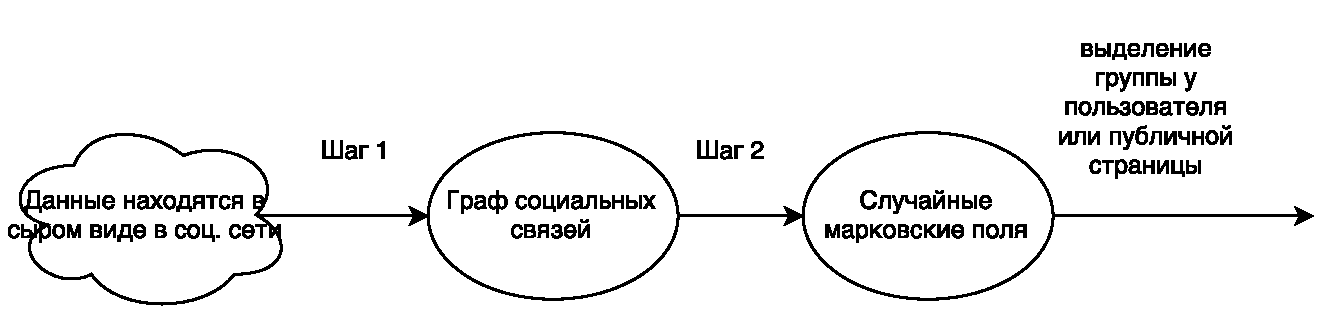
\includegraphics[width=\textwidth]{figs/plan.pdf}
\end{figure}

Опишем последовательно схему представляемого подхода. Из поставленной задачи мы имеем проблему определение группы пользователей. И так, на первом этапе исходя из тематики группы необходимо собрать набор публичных страниц придерживающихся данной тематики. Для этого предлагается сделать аналог лингвистической экспертизы. 

Имея набор групп определенной тематики, мы собираем всю информацию связанную с этим группами: тексты подписчики и так далее, подробнее в разделе 4.2.

Собрав все необходимые данные строим по ним граф социальных связей с дополнительной информацией, подробнее в разделе 4.1 (шаг 1).

Преобразуем наш граф к модификации случайного марковского поля, используя дополнительную информацию, подробнее в разделе 4.3 (шаг 2).

\section{Граф социальных связей}
Для хранения собранных данных и представления их в удобном виде используется граф социальных связей.
Узлом графа может являться публичная страница или же сам пользователь. Ребро обозначает подписку на публичную страницу или двусторонние отношения определяемые как взаимная подписка или отношение ~--- дружба. На рисунке ~\ref{fig:grapth} проиллюстрирована схема графа.

\begin{figure}[!h]
\caption{Граф социальных связей}
\label{fig:grapth}
\centering
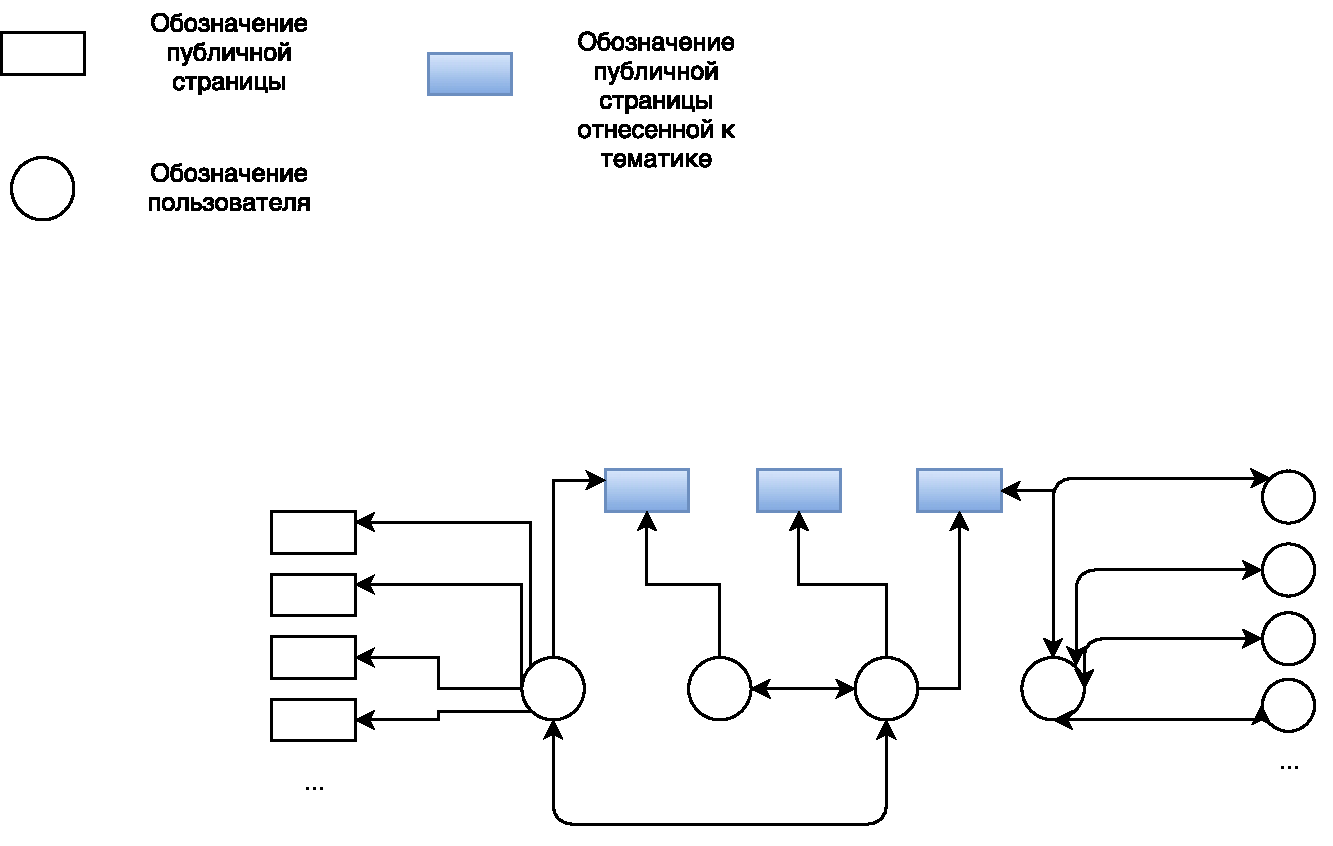
\includegraphics[width=\textwidth]{figs/graph.pdf}
\end{figure}

Узел группы содержат о себе следующую информацию: уникальный идентификатор, список публичных администраторов, список постов группы и для каждого поста, список одобривших его. На рисунке ~\ref{fig:public} проиллюстрирована схема хранения публичной страницы.

\begin{figure}[!h]
\caption{Узел публичной страницы в графе}
\label{fig:public}
\centering
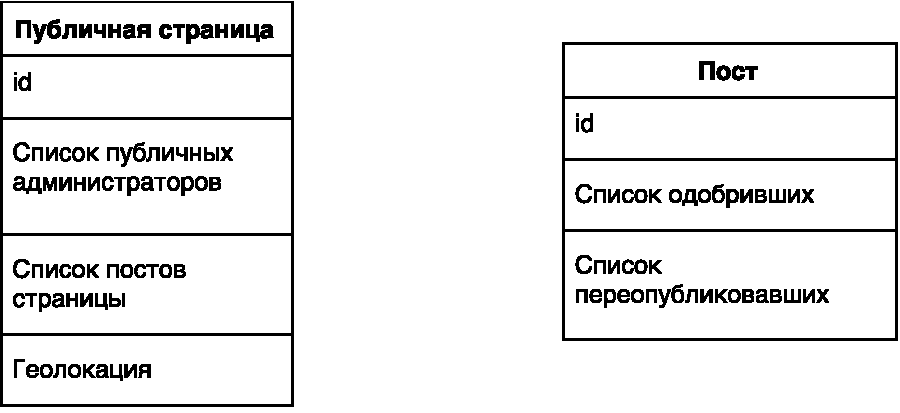
\includegraphics[width=\textwidth]{figs/public.pdf}
\end{figure}

Узел пользователя содержит о себе следующую информацию: уникальный идентификатор, фамилия, имя, текущая геолокация. На рисунке ~\ref{fig:user} проиллюстрирована схема хранения пользователя.

\begin{figure}[!h]
\caption{Пользовательский узел в графе}
\label{fig:user}
\centering
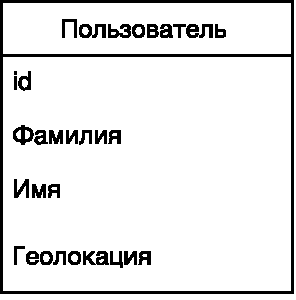
\includegraphics[width=0.3\textwidth]{figs/user.pdf}
\end{figure}

\newpage
На рисункe изображена схема хранения узлов графа.    

\section{Сбор данных}
В настоящем эксперименте решается задача для группы футбольных болельщиков и подгруппы радикальных фанатов.

В рамках данного исследования используются данные из социальной сети Вконтакте\footnote{https://vk.com}. Особенностью данной социальной сети является наличие двух видов публикующих страниц: обычного пользователя и группы, иначе публичной страницы. Пользователи имеют связи одновременно с группами и другими пользователями, публичные странице же связаны только с пользователями. 

Как было отмечено выше, первым дело необходимо создать список публичных страниц тематики искомой группы. 
Для этого должны быть определeны четкие характеристики определяемой группы.

Для группы футбольных болельщиков это: группа должна быть посвящена определенному футбольному клубу, это определялась по текстовым сообщениям, если в них присутствовали новости о футбольной команде, страница входит в группу. Для исследования были взяты группа страниц посвященных футбольному клубу "Зенит". Для определения публичных страниц входящих в подгруппу радикальных фанатов из собранных групп выбирались те, которые  содержали негативные отзывы о командах соперников, ненормативные высказывания в адрес болельщиков других команд. Всего было собрано 211 групп посвещенных этой тематике, 10 из которых были о футбольных хулиганах.

Так как при сборе подписчиков и подписок с только что добавленных узлов, граф очень быстро растет. В рамках данного исследования не проводились эксперименты с большим числом обновлений выборки. Пользователи добавлялись не более 2 раз, группы не более 3.

\section{Использование алгоритмов}
В данном разделе описано применение модифицрованных алгоритмов случайных марковских полей, латентного семантического анализа. Приведены особенности реализации и использования данных методов.
\subsection{Применение случайных марковских полей}
Условия задачи ставят определенные ограничения на используемые методы. Так имеется крайне ограниченная выборка, состоящая из небольшого набора публичных страниц. Поэтому предлагается воспользоватьcя подходом схожим с предложенным в статье. Так мы сможем значительно увеличить объем наших данных, вместе с тем используя алгоритм предложенный в разделе 2.4 мы всегда сможем оценить качество наших результатов.

Для эксперимента было выбрано две модификации описанного в разделе 2.4 подхода. 
Определим эти модификации.

Множества признаков $H$ будет одинаковым для двух модификаций, однако, оно будет отличаться от типа узла. Как уже было сказано социальная сеть Вконтакте обладает двумя типами узлов. Для узла пользователя определим два признака: наличие одобрения содержимого из смежных публичных страниц, принадлежащих к группе, и влияние характеристик смежных узлов. Для групп же: текстовая схожесть с текстами из подгруппы и влияние характеристик смежных узлов.

Использование методов, основанных на данных смежных узлов, обусловлено предположением, что пользователь, имеющий больше социальных связей с членами подгруппы, с большей вероятность сам будет принадлежать к этой подгруппе.

Использование признака одобрения контента основывается на предположении, что пользователь одобривший что-то действительно склонен одобрять данного рода информацию.


Модификации будут отличаться вычислением влияния смежных узлов.

В первом случае F будет считаться так:
\[
    F_{user}(x) = isApproved(x) or \sum_{y \in M_{adjacents}}p_{y}/n_{notnullable} > 0.5 
\]
\[
    F_{publicpage}(x) = textSimilarity(x) or \sum_{y \in M_{adjacents}}p_{y}/n_{notnullable} > 0.5 
\]

Во втором, как линейная комбинация:
\[
    F_{group}(x) = (k_{1} * isApproved(x) + k_{2} * \sum_{y \in M_{adjacents}}p_{y}/n_{notnullable}) / (k_{1} + k_{2}) 
\] 
\[
    F_{group}(x) = (k_{3} * textSimilarity(x) + k_{4} * \sum_{y \in M_{adjacents}}p_{y}/n_{notnullable}) / (k_{3} + k_{4}) 
\] 


Так изначально имея набор групп с размеченной характеристикой принадлежности к подгруппе получаем гораздо большую выборку. 

Процесс пересчета стоит продолжать до некоего E. В нашем случае было взято 0.2 \%.
При использовании упрощенной модели, вычисляется норма Фробениуса первого рода. 
  
Норма Фробениуса первого рода получает максимальную разницу в матрицах.

В результате такого подхода вероятности для групп могут измениться относительно изначальных. Путем сравнения с изначальными данными можно проверить качество модели.
На каждом шагу увеличения выборки проверяем изначальные данные.


Далее идет обход графа социальных связей описанного в прошлой главе. На каждом этапе добавляются новые подписчики, только что добавленных узлов графа и подписки, если они у узла есть.

\subsection{Текстовая схожесть}
Пользователи и публичные страницы создают и публикуют текстовые сообщения. У пользователей они как правило закрыты правилами приватности от большинства пользователей. У публичных страниц публикации как правило открыты. 

В описываемом алгоритме текстовые сообщения являются одним из важнейших типов данных. 

Используя их предлагается получать информацию о том, схожи ли сообщества своим содержанием или нет.

Выше были описаны несколько подходов к определению тематики текста. Предлагается воспользоваться двумя из них: тривиальным подходом и латено-семантическим анализом. 

Известно, что группа футбольных фанатов имеет набор сленговых фраз, например: <<бомжи>> ~--- фанаты футбольного клуба Зенит или же жители Санкт-Петербурга, <<свиньи>> ~--- фанаты футбольного клуба Спартак\footnote{https://ru.wiktionary.org/wiki/Приложение:Сленг\_футбольных\_хулиганов}.

Как описано выше, тривиальный алгоритм, предполагает составление словаря. Предлагается для составления словаря фраз относящихся к подгруппе радикальных фанатов использовать словарь с сайта wikipedia.com из раздела <<Сленг футбольных фанатов>>.

Так же для определения текстовой схожести предлагается воспользоваться латенто-семантическим анализом, а именно алгоритм LSI. В ходе разметки обучающей выборки, появился набор текстов относящихся к радикальным сообществам и относящихся к обычным фанатским сообществам. При использовании LSI, предлагается использоваться сингулярное разложение на две темы.

Предварительно предлагается отбросить термины, встречающиеся реже двух раз. Это позволит отбросить опечатки. 

В результате чего получаем набор терминов относящихся к радикальным сообществам.   

В качестве классификатора используем метод опорных векторов. 
\section{Описание программной реализации}
Кратко опишем реализацию применяемого подхода, а так же использованные библиотеки и средства.

В первую очередь стоит сказать, что подход был реализован на языке Python 3.

Для сбора данных с сайта Vk.com использовалась библиотека Vk\footnote{https://pypi.python.org/pypi/vk}. Социальная сеть жестко ограничвает частые запросы в свое API. Поэтому для корректного сбора больших данных с Vk.com, пришлось сделать обертку над указанной библиотекой, которая позволила максимальной эффективно собирать данные. Одной из особенностей используемого API является разделение запросов на два типа: требующие токена, и не требующие.

Для методов, не требующих токены, был реализовано два подхода сбора данных. К таким методам например относится метод $groups.getMembers$\footnote{https://new.vk.com/dev/groups.getMembers}. Использовать такие методы можно, делая таймауты только при получении ошибки. Первая реализация ~--- ленивая, позволяющая отправлять запросы на сервера, только непосредственно при вычислениях и обычная ~--- более удобная в ходе эксперимента, в котором не было необходимост делать вычисления на лету.

Все необходимые методы, можно было использовать без токена. Добавление токена в редких случаях давало дополнительные данные в некоторых публичных страниц. Из-за слабого улучшения и возможных проблем с кармой, было принято решение не использовать токены.

Для хранения данных, собранных из социальной сети, использовалась ORM Peewee\footnote{http://docs.peewee-orm.com/en/latest/}, данные хранились в реляционной базе данных PostgreSql\{https://www.postgresql.org/}. 

Граф социальных связей был отдельно реализован так же на языке Python 3.

Для стемминга слов использовалось программное средство MyStem\footnote{https://tech.yandex.ru/mystem/?ncrnd=325}. Проверки текста на вхождение символов, не принадлежащих к алфавиту, и слов, встречающихся реже, чем один раз, были одельно реализованы.

Для работы с матрицами иcпользовалась библиотека numpy\footnote{https://pypi.python.org/pypi/numpy}.

Для обучения использовалась библиотека sqlearn\footnote{http://scikit-learn.org/stable/}.

Обход графа социальных связей, его модификации и прочее были отдельно реализованы.

\section{Выводы по главе 3}
В настоящей главе описано применение алгоритмов описанных в прошлой главе. Показаны несколько подходов к решению каждой из подзадач. Показаны мотивации их применения и так же предполагаемые результаты. 
\chapter{Результаты}
В данной главе описаны результаты эксперимента проведенного в рамках исследования для апробирования подхода.
\section{Способы измерения качества результата}
Для оценки качества результатов используется несколько методов оценки.

Важным критерием является корректное определение групп из обучающей выборки после нескольких этапов добавления новых узлов в граф социальных связей. 

Так же интересен результат для пользователей определенных как администраторы сообществ. До начала эксперимента считается, что они буду принадлежать к той же группе, что и сообщество.

Основным методом оценки был выбран метод кросс-валидации. Выбранные группы делились на 10 частей, 9 групп входили в обучающую выборку. Оставшаяся часть использовалась для тестирования. Процедура повторялась 10 раз, для каждой части.

Алгоритм работает в несколько шагов, так что целесообразно проверять качество работы на разных этапах.
\section{Оценка результатов}
В данном разделе приведены результаты применения различных вариаций алгоритмов на группе футбольных болельщиков и радикальных футбольных фанатов.

Так как в ходе исследования не было обнаружено аналогично поставленных задача, результаты подохода сравним с результатами тривиальных алгоритмов.
\subsection{Результаты тривиальной оценки схожести текстов}
Данный метод казался перспективным, за счет того, что подгруппы пользователей взятые в эксперимент обладали собственным сленгом. Однако оказалось, что 
применение сленга довольно популярно и термины из словаря сленговых выражений встречались как и в подгруппе, так и в группе. Что не позволило использовать данный метод. Средняя оценка точности не превышала 60 \%. Поэтому подробное рассмотрение результатов этого метода не целесообразно.

Однако используя латентый сементический анализ удалось добиться хорошего разделения текста по тематикам. Так на изображении ~\ref{fig:sem} желтыми точками обозначены термины из группы обычных фанатов, красные из радикальных, синие ~--- это точки фанатские группы, зеленые ~--- радикальные фанатские группы. 

На изображении данные для шести радикальных групп и шести нерадикальных. 
\begin{figure}[!h]
\caption{Разделение на тематики}
\label{fig:sem}
\centering
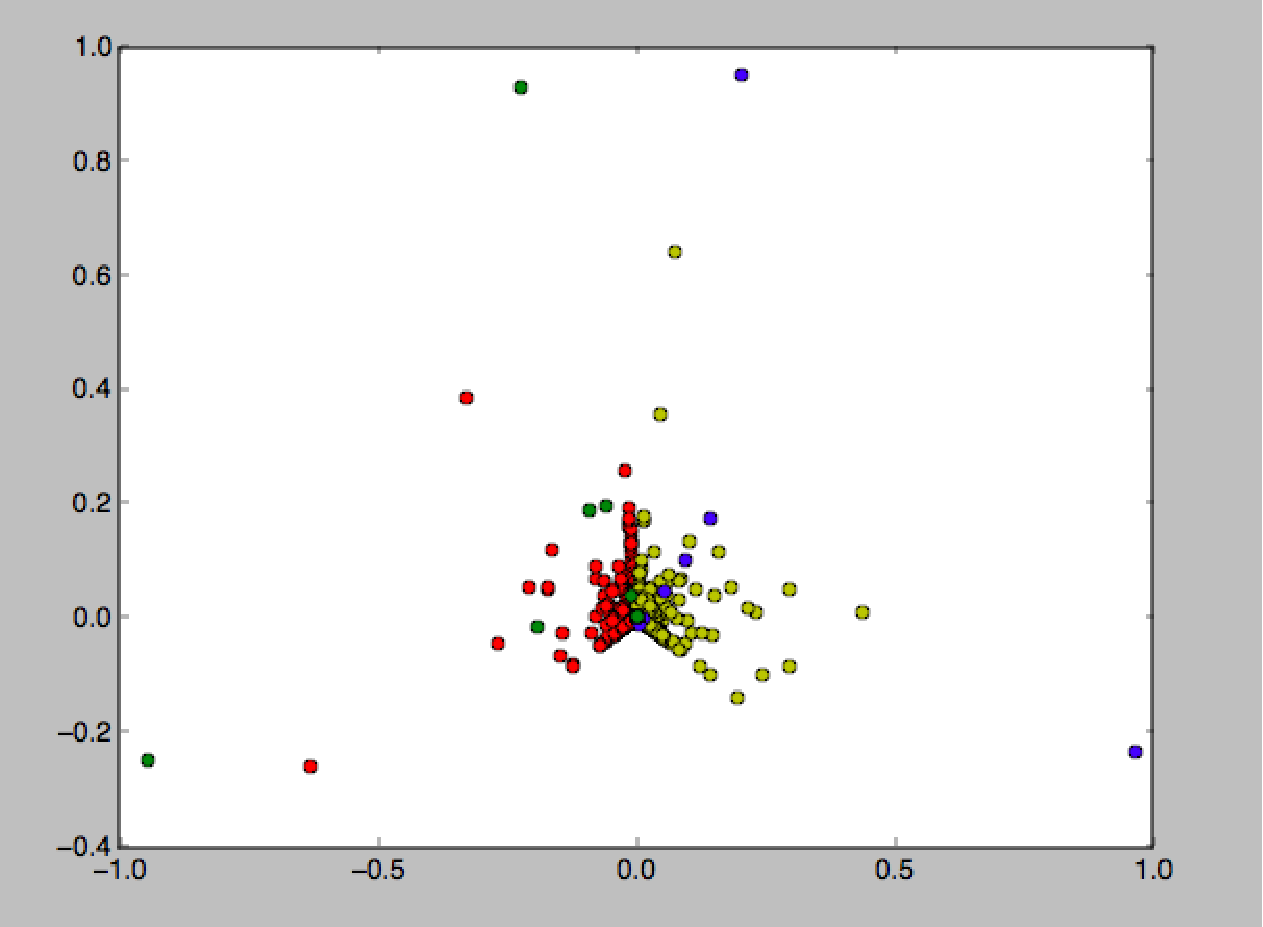
\includegraphics[width=\textwidth]{figs/sem.pdf}
\end{figure}

\newpage
\subsection{Тривиальные подходы}
Подход всегда определяющий узел как нерадикальный. 
При использовании подобного подхода, точность вычислений становится 95 \%. 
&f&-мера ~---

Подход определяющий узел как радикальный с вероятность 10 к 211.
\subsection{Результат метода оценки схожести основанного на операторе или}

Кросс-валидация дала следующие результаты {~\ref{tab2}}:

\begin{table}[!h]
\caption{Результат кросс валидации}\label{tab2}
\centering
\begin{tabular}{|*{11}{c|}}\hline
Номер выборки & 1 & 2 & 3 & 4 & 5 & 6 & 7 & 8 & 9 & 10 \\\hline
Точность  & 66\% & 66\% & 71\% & 62\% & 57\% & 57\% & 62\% & 57\% & 66\% & 62\% \\\hline
\end{tabular}
\end{table}

Средняя точность 63 \%. Данный метод показал плохой результат, возможно это связано с частым ложноположительным результатом, обоснованным слабой функцией схожести. Однако он не является достаточно показательным. Важным критерием является возможность определять членов подгруппы. Так как за счет не сбалансированности размеров классов, алгоритм, возвращающий наиболее часто встречающийся результат будет давать точность лучшую с увеличением класса. Точность же определения подгруппы будет 0.

$f_{1}$ мера для случайного распределения, где вероятность посчитать узел принадлежащим к подгруппе 50 \% : 1/11.

Посчитаем $f_{1}$ меру ~\ref{tab3}.

\[
    f_{1} = 2 * precision * recall / (precision + recall)
\] 

\begin{table}[!h]
\caption{Результат кросс валидации}\label{tab3}
\centering
\begin{tabular}{|*{11}{c|}}\hline
Номер выборки & 1 & 2 & 3 & 4 & 5 & 6 & 7 & 8 & 9 & 10 \\\hline
Recall  & 1& 1& 1& 1& 1& 1& 1& 1& 1& 1\\\hline
Precision & 1/7 & 1/7& 1/6& 1/8& 1/9& 1/9& 1/8 & 1/9& 1/7& 1/8\\\hline
F1 & 1/4 & 1/4 & 2/7 & 2/9 & 1/5 & 1/5 & 2/9 & 1/5 & 1/4 & 2/9 \\\hline

\end{tabular}
\end{table}

Алгоритм показывает очень сильный recall, однако из-за обилия ложноположительных результатов, precision очень низкий. F-мера довольно сильно превышает такую же меру для случайного результата.
 

Что касается сохранения точности при расширении выборки, при использовании данного метода размеченные в ручную публичные страницы никогда не помечались с ошибкой.

\subsection{Результат метода оценки схожести основанного на линейной комбинации}
Эксперименты проводились с несколькими значениями параметров. Однако были выбраны $k_{текстовой схожести} = 1$, $k{влияние харрактеристик смежных узлов}=1$, $k_{одобрение содержимого}=5$,  
кросс-валидация дала следующие результаты~\ref{tab1}:
\begin{table}[!h]
\caption{Результат кросс валидации}\label{tab1}
\centering
\begin{tabular}{|*{11}{c|}}\hline
Номер выборки & 1 & 2 & 3 & 4 & 5 & 6 & 7 & 8 & 9 & 10 \\\hline
Точность  & 90\% & 81\% & 85\% & 81\% & 76\% & 90\% & 85\% & 90\% & 85\% & 76\% \\\hline
\end{tabular}
\end{table}

Средняя точность 84 \%. По этой характеристике результат по прежнему слабый. Всегда определять узел как неотносящий к подгруппе выгоднее.

\begin{table}[!h]
\caption{Результат кросс валидации}\label{tab4}
\centering
\begin{tabular}{|*{11}{c|}}\hline
Номер выборки & 1 & 2 & 3 & 4 & 5 & 6 & 7 & 8 & 9 & 10 \\\hline
Recall  & 1& 1& 1& 1& 1& 1& 1& 1& 1& 0\\\hline
Precision & 1/2 & 1/4 & 1/3 & 1/4 & 1/5 & 1/2 & 1/3 & 1/2 & 1/3 & 0\\\hline
F1        & 2/3 & 2/5 & 1/2 & 2/5 & 1/3 & 2/3 & 1/2 & 2/3 & 1/2 & 0 \\\hline

\end{tabular}
\end{table}

$f$ мера показывает хороший результат~\ref{tab4},но в одном из номеров выборки она дала ложноотрицательный выбор. Это связано с тем, что появилось возможность поступательного уменьшения характеристики.
\chapterconclusion
В данной главе был описан эксперимент, проведенный в рамках исследования для апробации описываемого подхода.

На примере задачи определения подгрупп радикальных футбольных фанатов из группы футбольных болельщиков была показана состоятельность данного подхода. 

Выяснилось, что тривиальная оценка схожести может работать на определенных данных, однако имеет большую сложность в связи с необходимость составления правильного словаря для подгруппы. При неточном его составлении, качестве результатов сильно падает. Исследуемая модель показывает рост точности с использованием большего числа шагов, а значит большего числа узлов графа. 

Использование латенто-семантического анализа дало возможность улучшить результаты.

Предложенный подход с использованием оценки схожести, основанной на операторе или дал много ложноположительных определений членов подгруппы, однако показал абсолютную полноту.

При использовании оценки схожести основанной на линейной комбинации получается максимальная точность.

Предположение о том, что администраторы публичных страниц будут принадлежать подгруппе своих страниц, не подтвердилось. 

Предложенный подход позволяет достигнуть результатов на порядок лучших чем при случайном выборке.  
 Данный подход позволяет при наличии малой обучающей выборки получать приемлемый результат.



%% Макрос для заключения. Совместим со старым стилевиком.
\startconclusionpage

В данной работе был продемонстрирован подход, позволяющий определять принадлежат ли публичные сообщества и пользователи к подгруппе групп пользователей интернет-ресурсов имeющих социальную составляющую.

В ходе эксперименты выделялась подгруппа радикальных фанатов из группы болельщиков футбольного клуба Зенит. Результаты показали, что наилучшего результата удалось добиться с использованием подхода, использующего латентно-семантический анализ и линейную комбинацию признаков.

Стоит отметить, что предложенный подход выделения подгруппы пользователей, может использовать не представленные в исследовании признаки схожести. Кроме текстовых данных могут использоваться данные о геолокации, данные из других социальных сетей, полученный по идентификатору указанному в профиле, данные из медиа контента, опубликованного пользователями и сообществами. 

Метод может быть применим к любым видам групп и подгрупп. Подобная универсальность не гарантирует точности для любых видов групп, т.к. некоторые группы могут быть асоциальны и вовсе иметь нестандартную модель социальных связей. Однако описанный подход может дать хорошие результаты для многих из них. С другой стороны используя метод основанный на линейной комбинации можно улучшить результаты, пересчитывая на обучающих данных коэффициенты признаков. 

Предложенные признаки дают высокую полноту, а при применении других алгоритмов семантического анализа или других более точных алгоритмов получения тематики текста, возможно смогут дать более точное выделение подгруппы.

К сожалению не удалось сравнить результаты с другими подобными исследованиями, так как схожих постановок задачи не было обнаружено.

В числе недостатков предлагаемого метода: для описанных в примере признаков, качество результатов может сильно ухудшаться для некоторых видов подгрупп. Эта проблема решается введением новых признаков схожести.

В дальнейшем качество данного подхода можно улучшить добавлением дополнительных признаков, таких как например геолокация. Использование других модификаций случайных марковских полей так же может улучшить результат. Так же усоврешенствования существующих признаков тоже может улучшить результаты.

Интересен результат для большего числа шагов увеличения выборки.

Развитием данного подхода может послужить апробирование представленного метода на других группах и подгруппах.

%% Обратите внимание на heading. Без него тоже работает, но название будет другим.
\printbibliography[heading=trueHeading]

%% После этой команды chapter будет генерировать приложения, нумерованные русскими буквами.
%% \startappendices из старого стилевика будет делать то же самое
\appendix

\end{document}
